\section{实验结果}  % 原来是 \chapter

\subsection{训练参数}

\begin{table}[htbp]
\centering
\begin{tabular}{|l|l|}
\hline
\textbf{参数} & \textbf{取值} \\
\hline
batch\_size & 64 \\
epochs & 80 \\
初始学习率 & 0.001 \\
momentum & 0.9 \\
\hline
\end{tabular}
\caption{训练参数设置}
\label{tab:params}
\end{table}

\subsection{训练过程现象}

\begin{itemize}
\item 初期 loss 快速下降,accuracy 迅速提升至 95\%+
\item 后期收敛变慢,学习率衰减提高稳定性
\end{itemize}

\subsection{最终结果}

\begin{itemize}
\item 训练集准确率：约 99\%+
\item 测试集准确率：约 98\%+
\end{itemize}

\subsection{训练过程可视化}

训练过程中的 Loss 曲线、Accuracy 曲线和 Learning Rate 曲线如图所示。

\begin{figure}[htbp]
\centering
\begin{minipage}{0.3\textwidth}
\centering
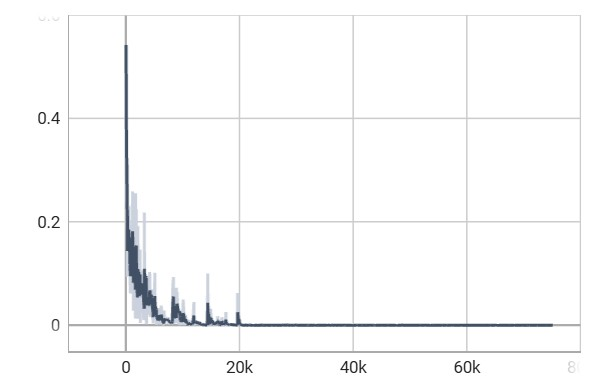
\includegraphics[width=\textwidth]{loss.jpg}
\caption{Loss 曲线}
\label{fig:loss}
\end{minipage}
\hfill
\begin{minipage}{0.3\textwidth}
\centering
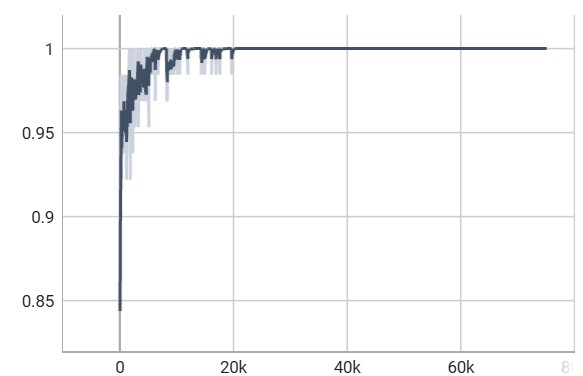
\includegraphics[width=\textwidth]{accuracy.jpg}
\caption{Accuracy 曲线}
\label{fig:accuracy}
\end{minipage}
\hfill
\begin{minipage}{0.3\textwidth}
\centering
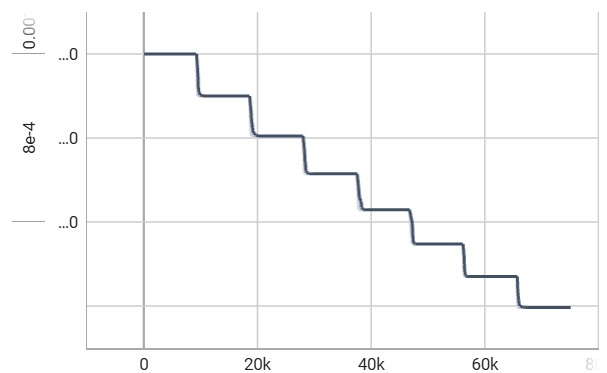
\includegraphics[width=\textwidth]{lr.jpg}
\caption{Learning Rate 曲线}
\label{fig:lr}
\end{minipage}
\label{fig:curves}
\end{figure}